\documentclass{siproblemset}

\usepackage{multicol}
\usepackage{xcolor}
\usepackage{mathtools}
\usepackage{enumitem}

% SI Session Information
\course{MTH 1321}
\sessionnum{FR}
\sessiondate{4/29/21}

% Worksheet Information
\title{Final Exam Practice Problems}
\withnamespace

\definecolor{darkred}{RGB}{110,0,0}
\raggedcolumns

%\debugmode

\begin{document}
    \maketitle
    
    \begin{center}
        \framebox{
            \begin{minipage}{\textwidth}
                \begin{center}
                    \textbf{This list of problems is not intended to be comprehensive of\linebreak all the material on your exam, but it should be good practice.}
                \end{center}
                \begin{enumerate}[leftmargin=*]
                    \item This list consists of homework questions which I consider to be representative of the important topics of each section.
                    \item Work through some or all of these leading up to your exam.
                    \item This list is intended to be \underline{supplemental} to your own exam review. Please do not only use this and the practice test to study for your exam.
                \end{enumerate}
            \end{minipage}
        }
    \end{center}
    
    \mcq{For the function $f(x)=3x+6$, compute the following questions:}{
        \task the average rate of change in the interval $[-3,-2]$
        \task the instantaneous rate of change at $x=-3$
        \task the slope of the secant line between $x=-3$ and $x=-2$
        \task the slope of the tangent line at $x=-3$
    }
    \mcq{For the function whose graph is given below, determine, for the given $x$-values if the two-sided limit exists and what its value is. Otherwise, find the left- and right-handed limits.}{
        \task $-3$
        \task $-1$
        \task $2$
        \task $4$
    }
    \begin{center}
        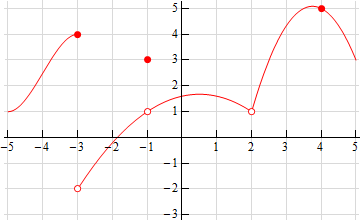
\includegraphics[width=0.7\linewidth]{FR02}
    \end{center}
    \mcq{Given $\lim\limits_{x\to 8}f(x)=-9$, $\lim\limits_{x\to 8}g(x)=2$, and $\lim\limits_{x\to 8}h(x)=4$, use the properties of limits to compute the following. Show your work.}{
        \task $\lim\limits_{x\to 8}\left[2f(x)-12h(x)\right]$ 
        \task $\lim\limits_{x\to 8}\left[g(x)h(x)-f(x)\right]$ 
    }
    \mcq{Compute the following limits, if they exist.}{
        \task $\lim\limits_{x\to 3}\dfrac{9}{(x-3)^5}$
        \task $\lim\limits_{t\to 8}\dfrac{t(t-5)}{t^2-8t}$
        \task $\lim\limits_{t\to 25}\dfrac{5-\sqrt{t}}{t-25}$
        \task $\lim\limits_{t\to 7}\dfrac{\frac17-\frac1x}{x-7}$
    }
    \mcq{Compute the following limits, if they exist.}{
        \task $\lim\limits_{x\to \infty}\dfrac{8-4x^2}{9x^2+5x}$
        \task $\lim\limits_{t\to \infty}\dfrac{\sqrt{7+9x^2}}{1-2x}$
        \task $\lim\limits_{t\to\infty}\dfrac{e^{2t}}{1-e^{-t}}$
        \task  $\lim\limits_{t\to-\infty}\dfrac{e^{2t}}{1-e^{-t}}$
    }
    \frq{Find the horizontal asymptotes of $f(x)=\dfrac{8-4x^2}{9x^2+5x}$.}
    \frq{Where is the function $f(x)=\dfrac{6}{z^2-3z-10}$ discontinuous?}
    \frq{Use the Intermediate Value Theorem to show that the given equation has at least one solution on the specified interval. $$25-8x^2-x^3=0~~~~~[-2,4]$$}
    \frq{Use the limit definition of the derivative to compute $f'(2)$ for $f(x)=x^2$.}
    \frq{Use the limit definition of the derivative to compute $f'(1)$ for $f(x)=\sqrt{3x-4}$.}
    \frq{Compute $\dddx[y]$ for $4x^2y^7-2x=x^5+4y^3$.}
    
\end{document}